\subsection{Results and discussion}
\phantomsection

\subsubsection{Reducing the size of chemical libraries}

To create a new version of the in-house (IRB) chemically diverse compound library, the primary task was to select representative small molecules from various vendors. Given the diverse research and biological experiments conducted at the institute, the constructed library should cover a broad range of the chemical space. For instance, the selection included both fragments (having low molecular weight) and compounds known to act through covalent binding, among others. 

Of particular interest was the inclusion of compounds from the ChemDiv commercial library (\hyperlink{https://www.chemdiv.com/}{https://www.chemdiv.com/}), a leading provider of small molecules for drug discovery. First, we filtered the 1.5M compounds included in the ChemDiv catalog based on various criteria (e.g. discarding highly lipophilic compounds, see \hyperref[Navigation_Methods]{Methods}). Following the filtering process, 559k compounds remained, which was an order of magnitude higher than the intended size of the ChemDiv selection for the IRB library. In light of this, we implemented a clustering strategy, with the aim of preserving the chemical diversity of the overall set, rather than relying on a random selection of compounds. In brief, after characterizing all small molecules with chemistry-based CC signatures (see Fig \ref{Navigation_Fig1}a, b, d and e for A1, A2, A3 and A4 signatures’ applicability values, respectively), we clustered numerical vectors using the K-means algorithm, setting the number of clusters to 35,000 (see \hyperref[Navigation_Methods]{Methods}). In fact, 328 of the clusters only included a single small molecule, while 51 of them contained 60 or more compounds (Fig \ref{Navigation_Fig1}c). The tSNE representation of all signatures revealed that compounds within the most populated clusters were closely placed together in the compressed 2D space, illustrating the coherence of the clustering outcomes (Fig \ref{Navigation_Fig1}f). To further validate our results, we assessed the standard deviations of signature features within each cluster, finding that the obtained values were consistently lower than those from random selections of compounds (Fig \ref{Navigation_Fig1}g). Finally, for each cluster, we calculated the distances between the cluster centroid (an abstract 512-dimensional point, see \hyperref[Navigation_Methods]{Methods}) and the nearest compound, the farthest compound and the remaining compounds within the cluster, and a subset of compounds from other clusters. As expected, we observed that the distances between the centroid and the compounds within each cluster were consistently shorter than those between the centroid and compounds from other clusters (Fig \ref{Navigation_Fig1}k, o). 

Finally, to select a balanced sample of each cluster, we selected the compounds that were closest and farthest from the cluster centroid as the cluster representatives. For clusters containing only a single compound, that compound was selected accordingly. All compounds selected as cluster representatives were subsequently chosen as ChemDiv representatives and thus included in the updated version of the IRB library, totalling 69,672 small molecules. Notably, the ChemDiv representatives exhibited physicochemical properties comparable to those of the entire ChemDiv library after filtering (Fig \ref{Navigation_Fig1}h-j and Fig \ref{Navigation_Fig1}l-n). 

%%%%%%%%%%%%%%%%
%%% FIGURE 1 %%%
%%%%%%%%%%%%%%%%

\begin{Figure_modified}
  \centering
  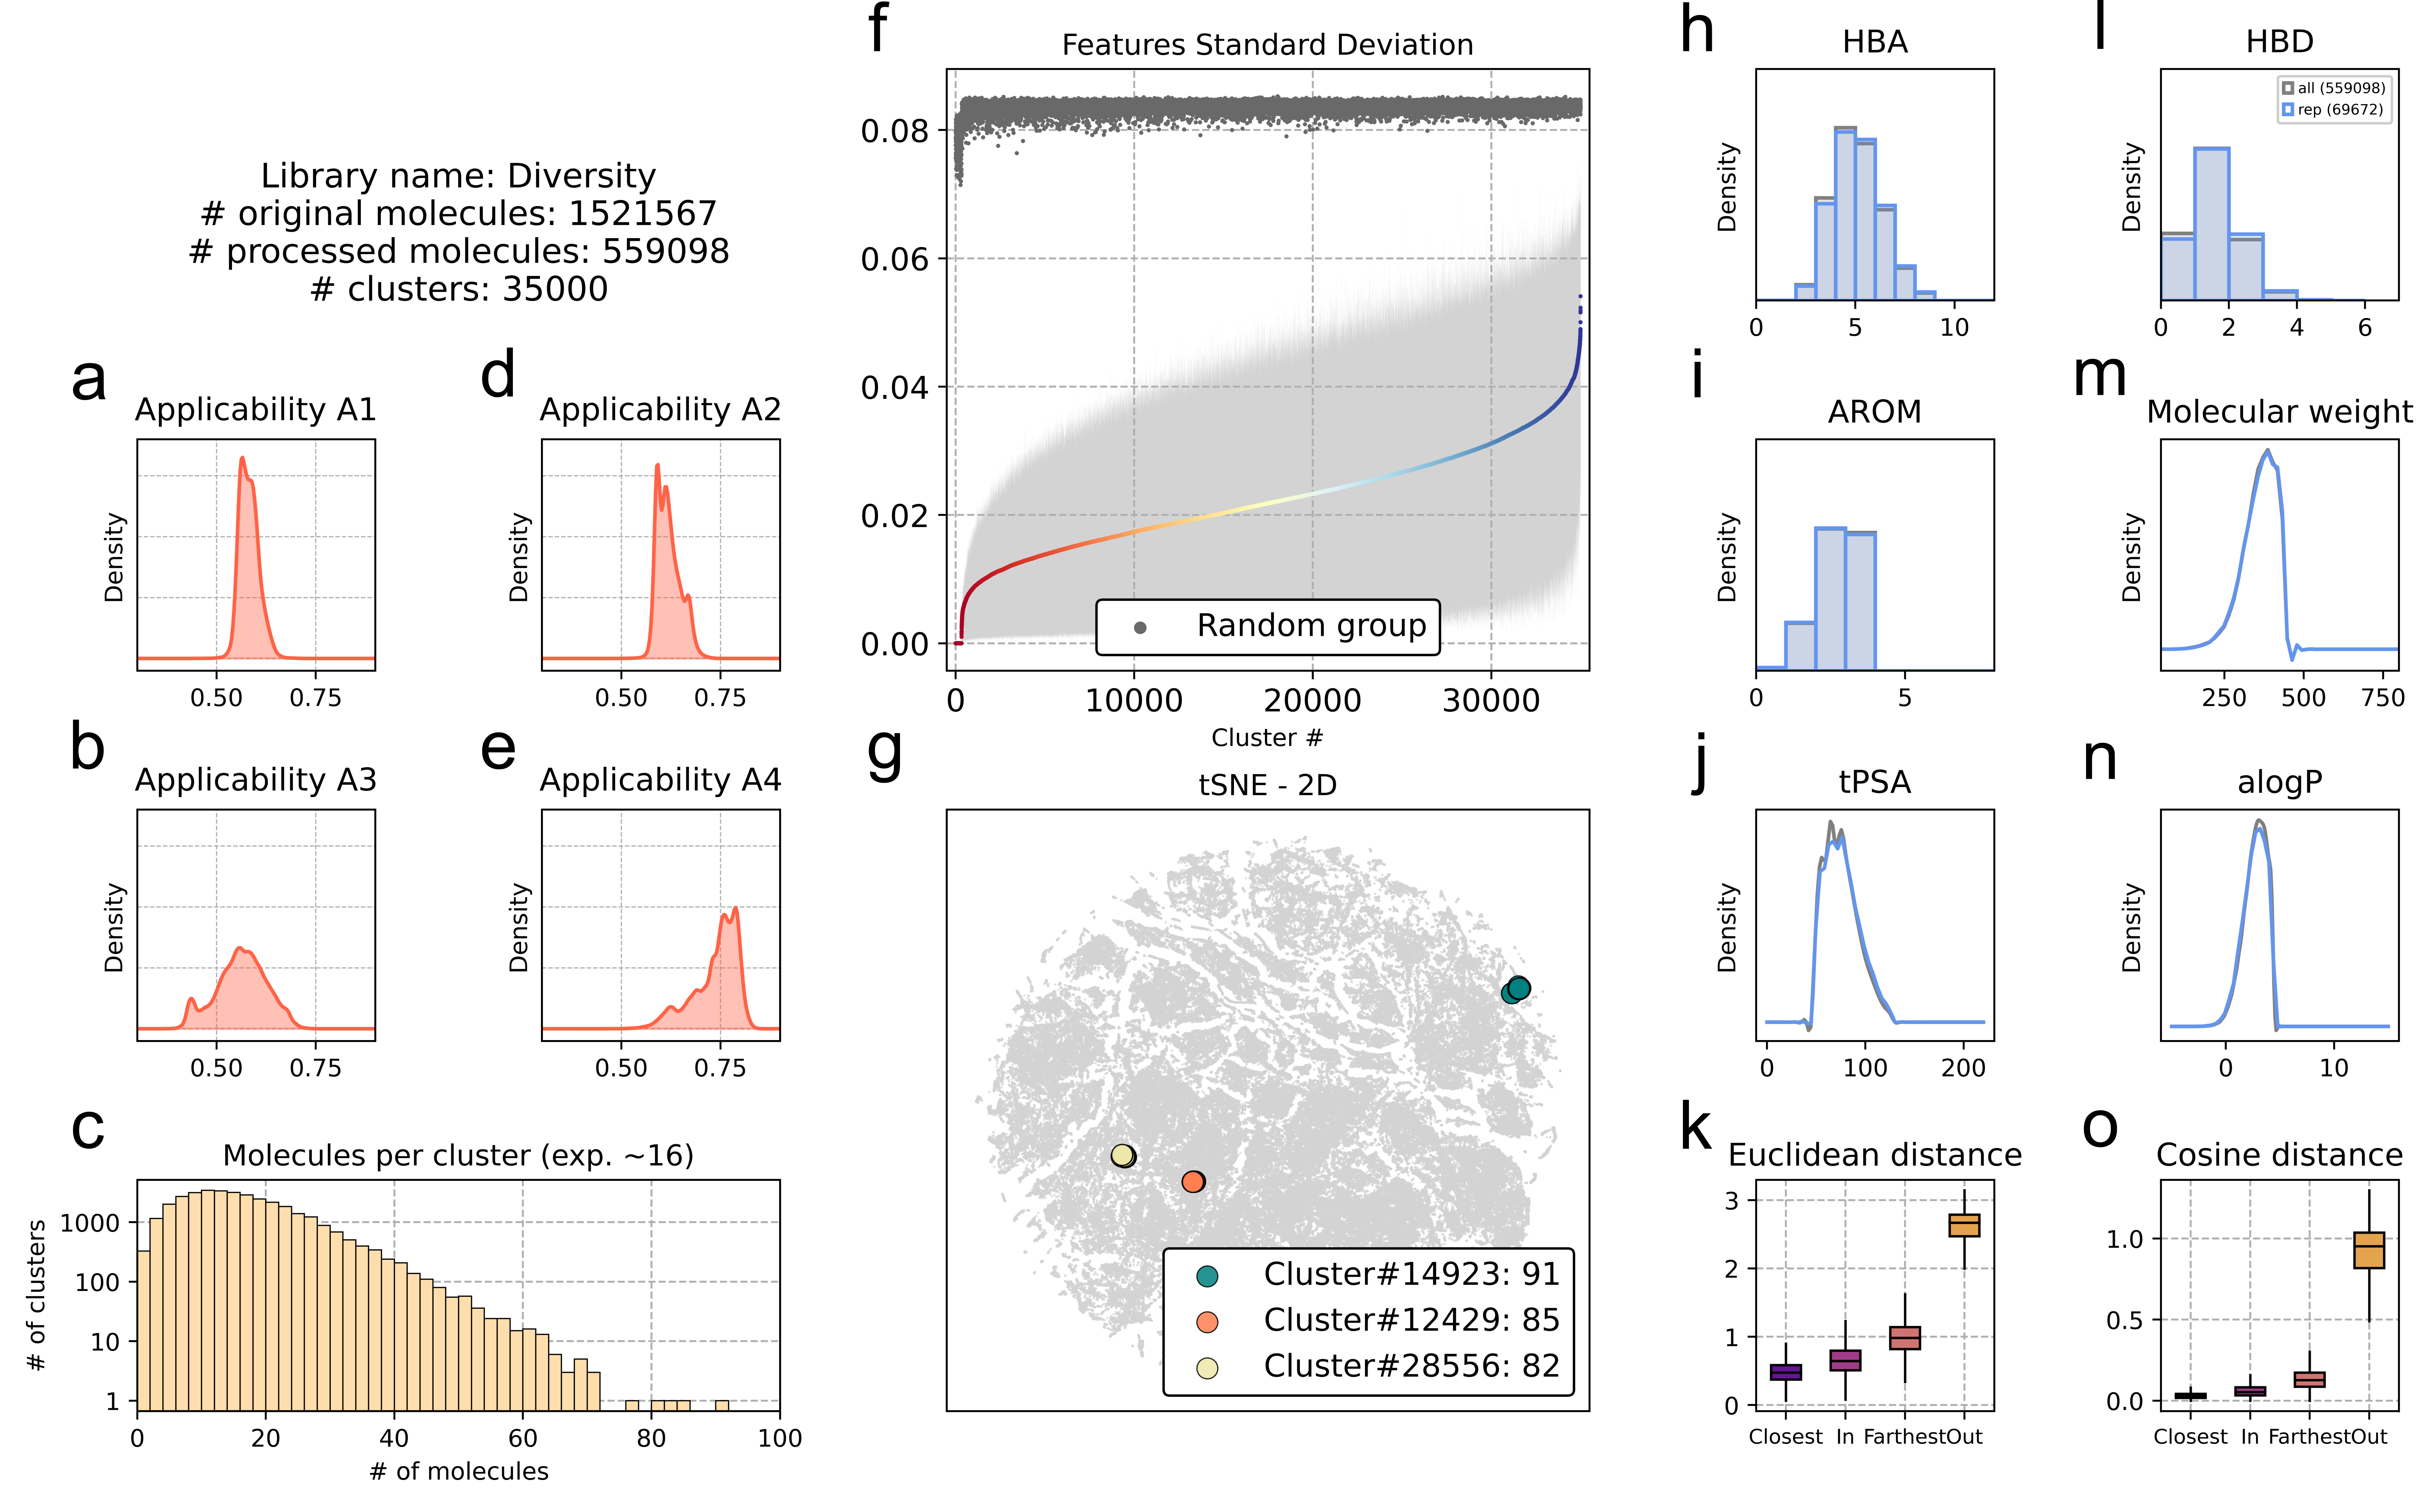
\includegraphics[width=1\linewidth]{figures/Navigation/Main/Diversity_random_v3.png}
  \caption{\textbf{Clustering a chemical library of compounds.}
    \textbf{a,b,d,e)} Distribution of CC signatures’ applicability values for A1, A2, A3 and A4, respectively. 
    \textbf{c)} Number of clusters (y-axis, log scale) having the specified number of molecules (x-axis). The expected number of molecules per cluster is 559k/35k \textasciitilde 16.
    \textbf{f)} For each cluster (x-axis, labeled from 0 to 34,999) standard deviations (y-axis) of the 128 features. Colored points represent the average standard deviation values of the features from signatures within the cluster, light gray bars show the range between the 20\textsuperscript{th} and 80\textsuperscript{th} percentiles of the distribution. Dark gray points represent the average standard deviation values of the features from randomly selected signatures outside the cluster.
    \textbf{g)} 2D tSNE representation of the 559k signaturized compounds (see \hyperref[Navigation_Methods]{Methods}). The top3 most populated clusters are colored accordingly, the legend indicates the number of small molecules within each of these clusters.
    \textbf{h,i,j,l,m,n)} Distributions of number of hydrogen bond acceptors, hydrogen bond donors, aromatic rings, molecular weight, topological polar surface area (tPSA) and alogP for the 559k ChemDiv compounds (after filtering, gray color) and the \textasciitilde70k selected representatives (light blue).
    \textbf{k,o)} Cosine and euclidean distances between the cluster centroid (an abstract 512-dimensional point, see \hyperref[Navigation_Methods]{Methods}) and the nearest compound, the farthest compound and the remaining compounds within each cluster, and a subset of compounds from other clusters.
}
  \vspace{-5mm}
  \rule[0ex]{\textwidth}{0.5pt}
  \vspace{-9mm}
  \label{Navigation_Fig1}
\end{Figure_modified}

\subsubsection{Qualitative visualization of the Chemical Space of small molecules}

To abstractly illustrate the chemical space of small molecules we subsampled compounds from Medina, Metabolights \cite{yurekten_metabolights_2024, haug_metabolights_2019}, CMAUP \cite{zeng_cmaup_2019, hou_cmaup_2024}, RepoHub \cite{corsello_drug_2017}, the Chemical Checker database \cite{duran-frigola_extending_2020} and the in-house chemically diverse IRB Library (herein named Chemical Diversity. Note that we here used the old version of the IRB Library, including 47k compounds). Medina’s natural product library represents one of the largest microbial extract libraries worldwide, providing a unique and invaluable resource for bioactive compound discovery (\hyperlink{https://www.medinadiscovery.com/natural-products-collection/}{https://www.medinadiscovery.com/natural-products-collection/}). On a similar note, Metabolights includes annotated metabolic compounds from various species, while CMAUP provides detailed information on active ingredients of useful medicinal plants. On the other hand, RepoHub (i.e. the Drug Repurposing Hub) is composed of existing clinical and marketed drugs, and is mainly aimed at repurposing known drugs for new therapeutic applications. Additionally, the Chemical Checker database comprises compounds with reported bioactivity in the public domain, and finally, the old version of the IRB proprietary library was specifically designed to maximize chemical diversity, covering a broad area of the synthetic chemical space.

To depict chemical differences between small molecule libraries, we generated chemical CC signatures for all molecules under study (see \hyperref[Navigation_Methods]{Methods}). Such signatures were in fact compact versions (128 dimensions) of state-of-the art chemical fingerprints, including ECFPs (CC A1 space), E3FPs (CC A2), together with embedded Murcko’s scaffold-based representations (CC A3), MACCs Keys (CC A4) and general physicochemical properties (CC A5). Additionally, we also generated bioactivity signatures, i.e. inferred representations of protein binding profiles (CC B4). 

Overall, we observed significant differences in the covered areas of the chemical space when using chemical signatures (A1-A5). For instance, there was very little overlap between compounds from the Chemical Diversity library and natural products from the Medina set (Fig \ref{Navigation_Fig2}). As expected, MetaboLights and CMAUP partially overlapped with Medina, while RepoHub and the Chemical Checker tended to extensively overlap with synthetically diverse compounds. The use of bioactivity signatures (B4) led to the analogous conclusion: natural products and synthetic drugs exhibited distinct protein binding profiles (Fig \ref{Navigation_Fig2}). Indeed, designed drugs and synthetically created compounds are imperfect human inventions with suboptimal properties and bioactivities, usually leading to limited efficacy and undesirable off-target effects. On the other hand, natural products and other ingredients derived from nature have evolved under the pressures of natural selection, resulting in tailored properties and refined selectivity profiles largely owing to their intricate chemical structures. Indeed, the scaffolds covered by synthetic compounds were far simpler than those included in natural products (Fig \ref{Navigation_FigS3}). 



%%%%%%%%%%%%%%%%
%%% FIGURE 2 %%%
%%%%%%%%%%%%%%%%

\begin{Figure_modified}
  \centering
  \includegraphics[width=1\linewidth]{figures/Navigation/Main/ALL_PRETTY.png}
  \caption{\textbf{Chemical space visualization of 6 distinct chemical libraries:} Medina, MetaboLights\cite{yurekten_metabolights_2024, haug_metabolights_2019}, CMAUP\cite{hou_cmaup_2024, zeng_cmaup_2019}, Chemical Diversity, RepoHub\cite{corsello_drug_2017} and the Chemical Checker\cite{duran-frigola_extending_2020}. For each combination of small molecule descriptor (A1-A5 and B4 CC Spaces) and compound library, tSNE 2D representation of the 31,052 generated signatures (see \hyperref[Navigation_Methods]{Methods}). Points are colored by density.
}
  \vspace{-5mm}
  \rule[0ex]{\textwidth}{0.5pt}
  \vspace{-9mm}
  \label{Navigation_Fig2}
\end{Figure_modified}







%%%%%%%%%%%%%%%%
%%% FIGURE 3 %%%
%%%%%%%%%%%%%%%%

\begin{Figure_modified}
  \centering
  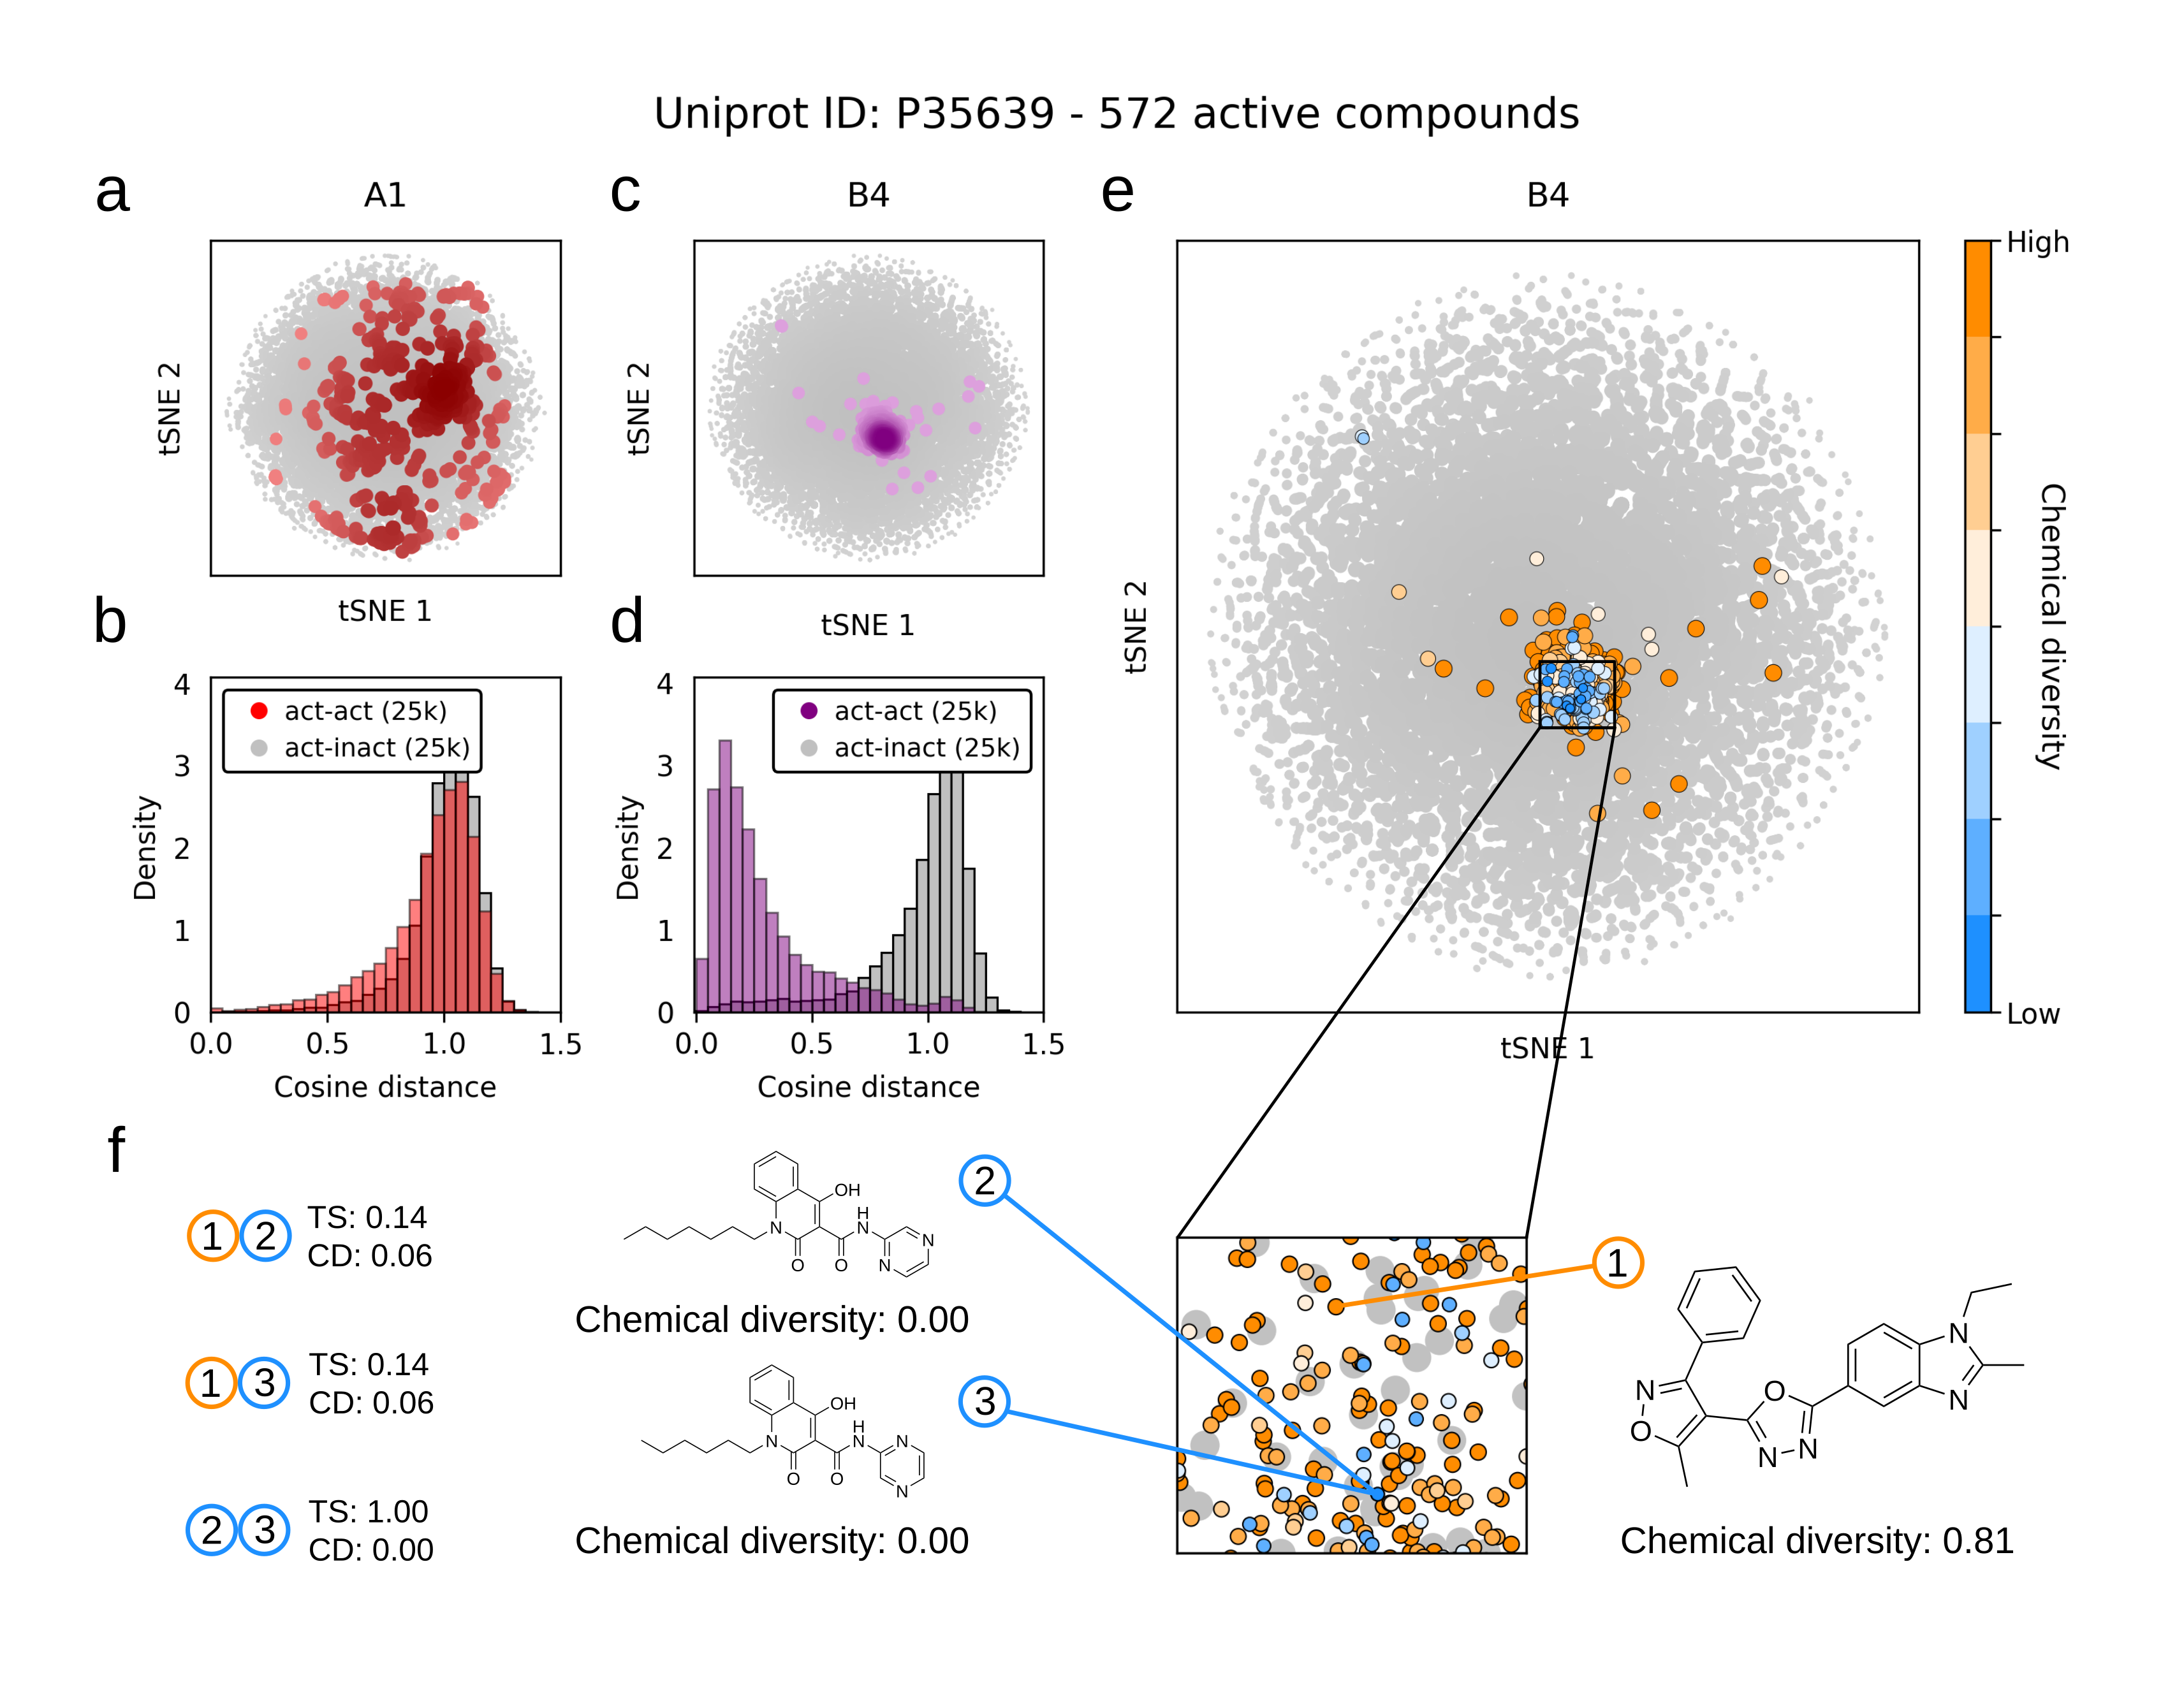
\includegraphics[width=1\linewidth]{figures/Navigation/Main/Fig3_v3.png}
  \caption{\textbf{The advent of bioactivity signatures.}
    \textbf{a)} tSNE 2D representation of the 572 compounds (red, colored by density) reported to be active against P35639 (Uniprot ID, Gene Name: DDIT3) in the CC database (v.2024) derived from ChEMBL and BindingDB. Gray dots correspond to 10k randomly selected compounds that serve as a background of the chemical space. All compounds were previously characterized using the CC A1 signaturizer\cite{bertoni_bioactivity_2021}.
    \textbf{b)} Distribution of cosine distances between active compounds (red, 25k subsampled comparisons) and between active and inactive compounds (gray, 25k subsampled comparisons). All compounds were previously characterized using the CC A1 signaturizer\cite{bertoni_bioactivity_2021}.
    \textbf{c)} tSNE 2D representation of the 572 compounds (purple, colored by density) reported to be active against P35639 (Uniprot ID, Gene Name: DDIT3) in the CC database (v.2024) derived from ChEMBL and BindingDB. Gray dots correspond to 10k randomly selected compounds that serve as a background of the chemical space. All compounds were previously characterized using the CC B4 signaturizer\cite{bertoni_bioactivity_2021}.
    \textbf{d)} Distribution of cosine distances between active compounds (purple, 25k subsampled comparisons) and between active and inactive compounds (gray, 25k subsampled comparisons). All compounds were previously characterized using the CC B4 signaturizer\cite{bertoni_bioactivity_2021}.
    \textbf{e)} tSNE 2D representation of the 572 compounds (colored by chemical diversity, see Methods) reported to be active against P35639 (Uniprot ID, Gene Name: DDIT3) in the CC database (v.2024) derived from ChEMBL and BindingDB. In short, the chemical diversity value represents the chemical redundancy from the neighboring environment of a bioactivity signature. Gray dots correspond to 10k randomly selected compounds that serve as a background of the chemical space. All compounds were previously characterized using the CC B4 signaturizer\cite{bertoni_bioactivity_2021}.
    \textbf{f)} A defined region of the chemical space (see previous subplot) is zoomed in to show (i) a compound having a high chemical diversity value (orange) as well as (ii) a pair of compounds having low chemical diversity (high chemical redundancy, blue). TS: Tanimoto Similarity. CD: Cosine Distance. 
}
  \vspace{-5mm}
  \rule[0ex]{\textwidth}{0.5pt}
  \vspace{-9mm}
  \label{Navigation_Fig3}
\end{Figure_modified}